% ALATPay Streams — Build with ALATPay Buildathon pitch deck
% Compile with: xelatex deck.tex   (twice, for the progress bar)
\documentclass[aspectratio=169,11pt]{beamer}

\usetheme[progressbar=frametitle, numbering=fraction, block=fill]{metropolis}
\usepackage{fontspec}
\usepackage{booktabs}
\usepackage{tabularx}
\usepackage{tikz}

\definecolor{brand}{HTML}{2563EB}      % Royal Blue
\definecolor{brandsoft}{HTML}{93C5FD}  % light blue
\definecolor{ink}{HTML}{09090B}        % zinc-950
\definecolor{paper}{HTML}{FAFAFB}      % page background
\definecolor{muted}{HTML}{52525B}      % zinc-600
\definecolor{hairline}{HTML}{E4E4E7}   % zinc-200
\definecolor{mint}{HTML}{059669}       % emerald

\setbeamercolor{normal text}{fg=ink, bg=paper}
\setbeamercolor{alerted text}{fg=brand}
\setbeamercolor{example text}{fg=mint}
\setbeamercolor{frametitle}{fg=ink, bg=paper}
\setbeamercolor{progress bar}{fg=brand, bg=hairline}
\setbeamercolor{title separator}{fg=brand}
\setbeamercolor{progress bar in head/foot}{fg=brand, bg=hairline}
\setbeamercolor{progress bar in section page}{fg=brand, bg=hairline}
\setbeamercolor{block title}{fg=ink, bg=hairline!40!paper}
\setbeamercolor{block body}{fg=muted, bg=hairline!40!paper}

\setsansfont[BoldFont={Helvetica Neue Bold}, ItalicFont={Helvetica Neue Italic}]{Helvetica Neue}
\setmonofont{Menlo}

\setbeamerfont{frametitle}{size=\Large, series=\bfseries}
\setbeamerfont{title}{size=\Huge, series=\bfseries}

\newcommand{\mutedtext}[1]{{\color{muted}#1}}
\newcommand{\kpi}[2]{{\centering{\color{brand}\Huge\bfseries #1}\\[2pt]\mutedtext{\small #2}\par}}

\title{ALATPay Streams}
\date{}

\begin{document}

% ---------- 1 · Title (dark, like the site's hero) ----------
\begingroup
\setbeamercolor{background canvas}{bg=ink}
\setbeamercolor{normal text}{fg=white, bg=ink}
\usebeamercolor[fg]{normal text}
\begin{frame}[plain]
  % Custom background art for title cover
  \begin{tikzpicture}[remember picture, overlay]
    % Circular radial glow shifted to the right edge
    \shade[inner color=brand!20!ink, outer color=ink, opacity=0.95] 
      ([xshift=0.5cm, yshift=-0.5cm]current page.east) circle (5.5cm);
    
    % Stream flow nodes (scaled and shifted rightward to clear text)
    \begin{scope}[shift={([xshift=-1.6cm, yshift=0.5cm]current page.east)}, scale=0.62]
      \coordinate (A) at (-2.8, 0);
      \coordinate (B1) at (0, 1.4);
      \coordinate (B2) at (0, 0.45);
      \coordinate (B3) at (0, -0.45);
      \coordinate (B4) at (0, -1.4);
      
      % Draw spline connections
      \draw[brandsoft!45!ink, line width=2.5pt] (A) to[out=25, in=180] (B1);
      \draw[brand!60!ink, line width=2.5pt] (A) to[out=8, in=180] (B2);
      \draw[brandsoft!35!ink, line width=2.5pt] (A) to[out=-8, in=180] (B3);
      \draw[brand!50!ink, line width=2.5pt] (A) to[out=-25, in=180] (B4);
      
      % Flow dots on the streams
      \fill[brandsoft] ([xshift=-1.1cm]B1) circle (3pt);
      \fill[brand] ([xshift=-0.7cm]B2) circle (3.5pt);
      \fill[brandsoft] ([xshift=-1.8cm]B3) circle (3pt);
      \fill[brand] ([xshift=-1.3cm]B4) circle (3.5pt);
      
      % Nodes
      \fill[brandsoft] (A) circle (6.5pt);
      \fill[brand] (B1) circle (4.5pt);
      \fill[brand] (B2) circle (4.5pt);
      \fill[brand] (B3) circle (4.5pt);
      \fill[brand] (B4) circle (4.5pt);
    \end{scope}
  \end{tikzpicture}

  \vspace{1.8cm}
  {\Huge\bfseries Money in. Already {\color{brandsoft}sorted.}\par}
  \vspace{0.4cm}
  {\large\color{white!80!ink} Programmable income routing for Nigerian merchants, built on ALATPay.\par}
  \vfill
  {\color{white!50!ink}\scriptsize
    Team ALATPay Streams \;·\; Build with ALATPay Buildathon 2026
  \par}
  \vspace{0.8cm}
\end{frame}
\endgroup

% ---------- 2 · Problem ----------
\begin{frame}{The problem: every naira lands in one pool}
  \vspace{0.2cm}
  \begin{columns}[T]
    \begin{column}{0.58\textwidth}
      \begin{itemize}
        \item A merchant's sales, tax money, supplier money and salary all sit in \textbf{one account balance} — and get spent as one.
        \item VAT is a quarterly ambush. Suppliers are paid late. Savings never happen.
        \item The discipline is manual: notebooks, mental math, three phones.
      \end{itemize}
      \vspace{0.4cm}
      \mutedtext{Nigeria has \textbf{40M+ MSMEs}. Cash-flow indiscipline — not demand — is what kills most of them.}
    \end{column}
    \begin{column}{0.38\textwidth}
      \begin{alertblock}{The moment of failure}
        The money was there when it landed.\\It was gone when the bill arrived.
      \end{alertblock}
    \end{column}
  \end{columns}
\end{frame}

% ---------- 3 · Solution ----------
\begin{frame}{The fix: split every payment at source}
  {\large Every incoming payment is routed \textbf{the instant it lands} — before it can be spent.\par}
  \vspace{0.25cm}
  \begin{center}
    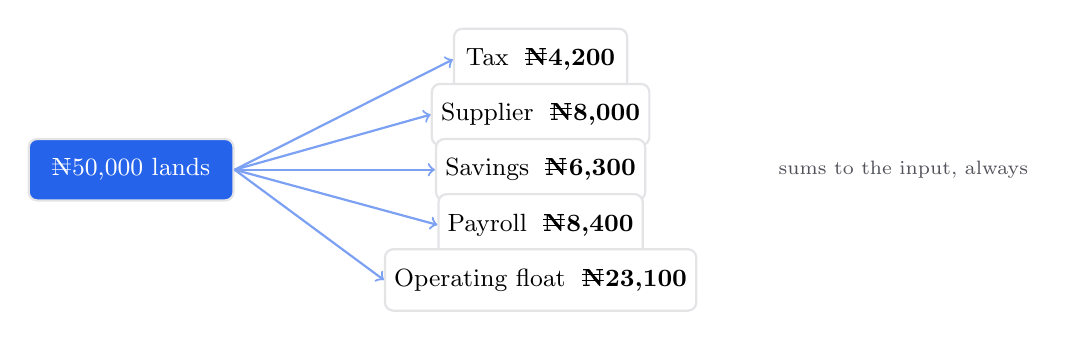
\begin{tikzpicture}[
      box/.style={draw=hairline, thick, rounded corners=3pt, fill=white,
                  minimum height=0.78cm, minimum width=2.2cm, font=\small},
      lbl/.style={font=\scriptsize\color{muted}}
    ]
      \node[box, fill=brand, text=white, minimum width=2.6cm] (in) at (0,0) {₦50,000 lands};
      \node[box] (tax)  at (5.2, 1.4) {Tax \;\textbf{₦4,200}};
      \node[box] (sup)  at (5.2, 0.7) {Supplier \;\textbf{₦8,000}};
      \node[box] (sav)  at (5.2, 0.0) {Savings \;\textbf{₦6,300}};
      \node[box] (pay)  at (5.2,-0.7) {Payroll \;\textbf{₦8,400}};
      \node[box] (op)   at (5.2,-1.4) {Operating float \;\textbf{₦23,100}};
      \foreach \t in {tax,sup,sav,pay,op} \draw[->, thick, brand!60!white] (in.east) -- (\t.west);
      \node[lbl, anchor=west] at (8.1, 0.0) {sums to the input, always};
    \end{tikzpicture}
  \end{center}
  \vspace{0.15cm}
  \begin{center}\mutedtext{The merchant never has to remember. The rules remember.}\end{center}
\end{frame}

% ---------- 4 · How it works ----------
\begin{frame}{How it works: one deterministic split engine}
  \vspace{0.2cm}
  \begin{center}
    {\large \textbf{Income lands} \;\alert{$\rightarrow$}\; \textbf{rules split} \;\alert{$\rightarrow$}\; \textbf{ledgers fill} \;\alert{$\rightarrow$}\; \textbf{AI acts}\par}
  \end{center}
  \vspace{0.4cm}
  \begin{columns}[T]
    \begin{column}{0.55\textwidth}
      \begin{enumerate}
        \item \textbf{FIXED} ledgers settle first, in strict priority
        \item \textbf{WEEKLY\_FIXED} fires only on its configured day
        \item \textbf{PERCENTAGE} ledgers share the remainder
        \item Whatever is left \(\rightarrow\) \textbf{operating float}
      \end{enumerate}
    \end{column}
    \begin{column}{0.41\textwidth}
      \begin{block}{Why deterministic}
        One pure function decides where every kobo goes. No AI in the money path — the co-pilot \emph{configures} rules, it never \emph{moves} funds.
      \end{block}
    \end{column}
  \end{columns}
\end{frame}

% ---------- 5 · Demo ----------
\begin{frame}{Live demo — two minutes}
  \vspace{0.2cm}
  \begin{enumerate}
    \item \textbf{Burst} — customer payments animate into ledgers \mutedtext{(one arrives via Tap \& Pay)}
    \item \textbf{Streams Voice} — \emph{``I just sold 80k today, business has been good this week''}
    \item \textbf{Loan offer} — the co-pilot answers with a pre-approved offer; we accept by voice
    \item \textbf{Streams Uptime} — \emph{``Your GTBank account — healthy, 99.1\% uptime. Sending ₦400,000 now.''}
  \end{enumerate}
  \vspace{0.4cm}
  \mutedtext{Everything on screen is running against the split engine and the ALATPay integration you're about to see.}
\end{frame}

% ---------- 6 · Three pillars ----------
\begin{frame}{The merchant counterpart to ALAT: The Evolution}
  \small
  \renewcommand{\arraystretch}{1.25}
  \begin{tabularx}{\textwidth}{@{}l X X@{}}
    \toprule
    \textbf{Pillar} & \textbf{Consumer (ALAT)} & \textbf{Merchant (Streams)}\\
    \midrule
    \textbf{Voice} & SAW voice banking & \alert{Streams Voice} — configure ledgers, check sales, accept loans by speaking\\
    \textbf{Contactless} & Tap and Pay & \alert{Tap \& Pay routing} — NFC payments split like any other channel\\
    \textbf{Predictive uptime} & Recipient bank availability & \alert{Streams Uptime} — rail health checked before every payout\\
    \bottomrule
  \end{tabularx}
  \vspace{0.25cm}
  \begin{center}
    \mutedtext{\emph{Wema built all three for consumers. We built them for merchants.}}
  \end{center}
\end{frame}

% ---------- 7 · Loans ----------
\begin{frame}{Streams Loans: underwritten by streams, not paperwork}
  \vspace{0.2cm}
  \begin{columns}[T]
    \begin{column}{0.55\textwidth}
      \begin{itemize}
        \item Scorecard runs on \textbf{90 days of routed income} — real revenue, already on our rails
        \item Offer surfaced in chat or voice; accepted in one sentence
        \item Repayment is \textbf{just another ledger} — deducted at source from every sale, so no missed instalments
      \end{itemize}
      \vspace{0.2cm}
      \mutedtext{\small Credit policy documented in \texttt{underwriting/MODEL.md} — ask us about it.}
    \end{column}
    \begin{column}{0.41\textwidth}
      \kpi{₦2,400,000}{pre-approved in the demo}
      \vspace{0.35cm}
      \kpi{6\%}{of daily income, deducted at source}
    \end{column}
  \end{columns}
\end{frame}

% ---------- 8 · Uptime ----------
\begin{frame}{Streams Uptime: we know a bank is down before your customer does}
  \vspace{0.2cm}
  \begin{itemize}
    \item Settlement rails scored continuously across Nigerian banks
    \item Checked \textbf{before} every loan disbursement and supplier payout
    \item Degraded rail? The transfer detours — no failed splits, no stranded funds
  \end{itemize}
  \vspace{0.5cm}
  \begin{exampleblock}{The demo line}
    ``Approved. Your account at GTBank — healthy, 99.1\% uptime today.\\
    Sending ₦400,000 now, expected to land in 4 seconds.''
  \end{exampleblock}
\end{frame}

% ---------- 9 · ALATPay integration ----------
\begin{frame}{Built on ALATPay — properly}
  \vspace{0.2cm}
  \begin{columns}[T]
    \begin{column}{0.52\textwidth}
      \textbf{Collection}
      \begin{itemize}
        \item Official SDK contract (\texttt{apibox.alatpay.ng})
        \item Virtual accounts · payment links · transaction status
      \end{itemize}
      \vspace{0.2cm}
      \textbf{Webhooks}
      \begin{itemize}
        \item HMAC signature verification (prod + staging header variants)
        \item Redis dedupe — retries land exactly once
      \end{itemize}
    \end{column}
    \begin{column}{0.44\textwidth}
      \textbf{Resilience}
      \begin{itemize}
        \item Idempotency keys on every payout
        \item Exponential backoff, 6s hard timeout
        \item Circuit breaker fails fast after 5 misses
      \end{itemize}
      \vspace{0.2cm}
      \mutedtext{\small Express 5 · TypeScript · Prisma/Postgres · Redis · Next.js dashboard}
    \end{column}
  \end{columns}
  \vspace{0.35cm}
  \begin{center}
    \mutedtext{\emph{Nine endpoints. That's the whole API.}}
  \end{center}
\end{frame}

% ---------- 10 · Why Wema ----------
\begin{frame}{Why this wins for Wema}
  \vspace{0.2cm}
  \begin{itemize}
    \item \textbf{ALATPay transaction data} becomes programmable income routing — a reason for merchants to keep volume on ALATPay rails
    \item \textbf{Defensible underwriting} on routed income opens SME credit with repayment at source
    \item \textbf{WhatsApp + voice co-pilot} reaches merchants who never open a laptop
    \item Wema distribution \;\(\times\)\; ALATPay rails \;\(\times\)\; Streams intelligence
  \end{itemize}
  \vspace{0.4cm}
  \mutedtext{Sticky deposits, richer data, credit-ready merchants — on infrastructure Wema already owns.}
\end{frame}

% ---------- 11 · Close (dark) ----------
\begingroup
\setbeamercolor{background canvas}{bg=ink}
\setbeamercolor{normal text}{fg=white, bg=ink}
\usebeamercolor[fg]{normal text}
\begin{frame}[plain]
  % Custom background art for the close slide (distribution/completion)
  \begin{tikzpicture}[remember picture, overlay]
    % Circular radial glow shifted to the right edge
    \shade[inner color=brand!20!ink, outer color=ink, opacity=0.95] 
      ([xshift=0.5cm, yshift=-0.5cm]current page.east) circle (5.5cm);
      
    % Stream flow nodes (scaled and shifted rightward to clear text)
    \begin{scope}[shift={([xshift=-1.6cm, yshift=0.5cm]current page.east)}, scale=0.62]
      \coordinate (A) at (-2.8, 0);
      \coordinate (B1) at (0, 1.4);
      \coordinate (B2) at (0, 0.45);
      \coordinate (B3) at (0, -0.45);
      \coordinate (B4) at (0, -1.4);
      
      % Draw spline connections
      \draw[brandsoft!45!ink, line width=2.5pt] (A) to[out=25, in=180] (B1);
      \draw[brand!60!ink, line width=2.5pt] (A) to[out=8, in=180] (B2);
      \draw[brandsoft!35!ink, line width=2.5pt] (A) to[out=-8, in=180] (B3);
      \draw[brand!50!ink, line width=2.5pt] (A) to[out=-25, in=180] (B4);
      
      % Flow particles moved near the endpoints (signifying routing complete)
      \fill[brandsoft] ([xshift=-0.25cm]B1) circle (3pt);
      \fill[brand] ([xshift=-0.08cm]B2) circle (3.5pt);
      \fill[brandsoft] ([xshift=-0.3cm]B3) circle (3pt);
      \fill[brand] ([xshift=-0.15cm]B4) circle (3.5pt);
      
      % Nodes
      \fill[brandsoft] (A) circle (6.5pt);
      \fill[brand] (B1) circle (4.5pt);
      \fill[brand] (B2) circle (4.5pt);
      \fill[brand] (B3) circle (4.5pt);
      \fill[brand] (B4) circle (4.5pt);
    \end{scope}
  \end{tikzpicture}

  \vspace{1.4cm}
  {\Huge\bfseries Every naira knows\\where it's going.\par}
  \vspace{0.8cm}
  {\large\color{white!80!ink}
  \textbf{Next:} live sandbox merchants \;·\; USSD for feature phones \;·\; agent banking\par}
  \vfill
  {\color{white!65!ink}\small ALATPay Streams \;·\; Build with ALATPay Buildathon 2026 \;·\; Thank you\par}
  \vspace{0.6cm}
\end{frame}
\endgroup

\end{document}
